\chapter{7}
\label{ch:7}

\section{Methodology}
From the API response, we extracted the date of the first and last snapshot and the total number of snapshots for each URI. 

\section{Results}
For both Software Heritage and Web archives, we calculated the time between the date of the first publication to reference a URI and the date of the first capture of the URI. Software Heritage was created on June 30, 2016 \cite{dicosmo_swhblog}, so we only analyzed articles that were published starting July 1, 2016. We found an average of 443 days (median of 360 days) between the first reference to the repository URI in a scholarly publication and the first capture by Software Heritage, if the repository-level URI did not have a snapshot at the time of publication. Additionally, 7,440 repository URIs that were captured before the publication date of the referencing article had not been captured since the article's publication. For these  URIs, there is an average of 253 days between the last Software Heritage snapshot and the publication date of the reference article. 

As shown in Figure \ref{fig:swh_delta},
the maximum time delta between the first reference to the repository URI in a scholarly publication and the first capture by Software Heritage has steadily decreased from 78 months for articles published in July 2016 to 9 months for articles published in April 2022. We also see that the median time delta follows a trend similar to the average time delta. The median and average time deltas have both decreased since 2021. 

\begin{figure}
    \centering
    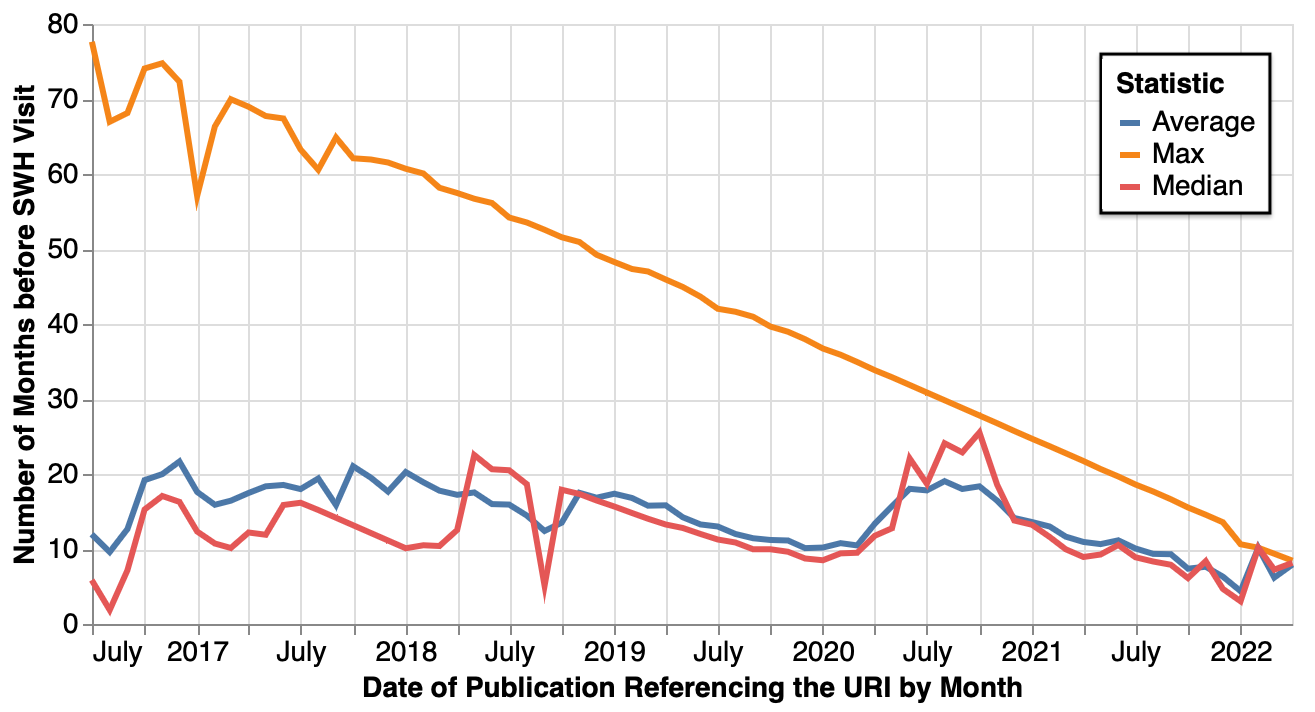
\includegraphics[width=0.85\linewidth]{SWH_delta_over_time.png}
    \caption{Months between a publication referencing a URI and the URI being captured by Software Heritage over time. Only includes URIs not been captured by Software Heritage before the publication date of the referencing article.}
    \label{fig:swh_delta}
\end{figure}

These trends for are similar for Web archives. There was an average of 468 days and a median of 341 days between the first reference to the URI in a scholarly publication and the first memento in a Web archive, if there were no mementos of the URI prior to the publication date of the referencing article. Of the URIs that had a memento in the Web archives prior to the publication date of the article, 4,356 URIs have not been archived since the article was published, with an average of 201 days between the latest memento and the publication date. Figure \ref{fig:timemap_delta} shows that the average and maximum time deltas have followed similar trends. Additionally, the maximum time delta has steadily decreased from 128 months in January 2012 to 1 month in April 2022. While the steady decline seen in maximum and average time deltas for Software Heritage and Web archives is promising, there is still a large period of time for the URI resource to move from  vulnerable to unrecoverable before Software Heritage or Web archives are able to archive it.

\begin{figure}
    \centering
    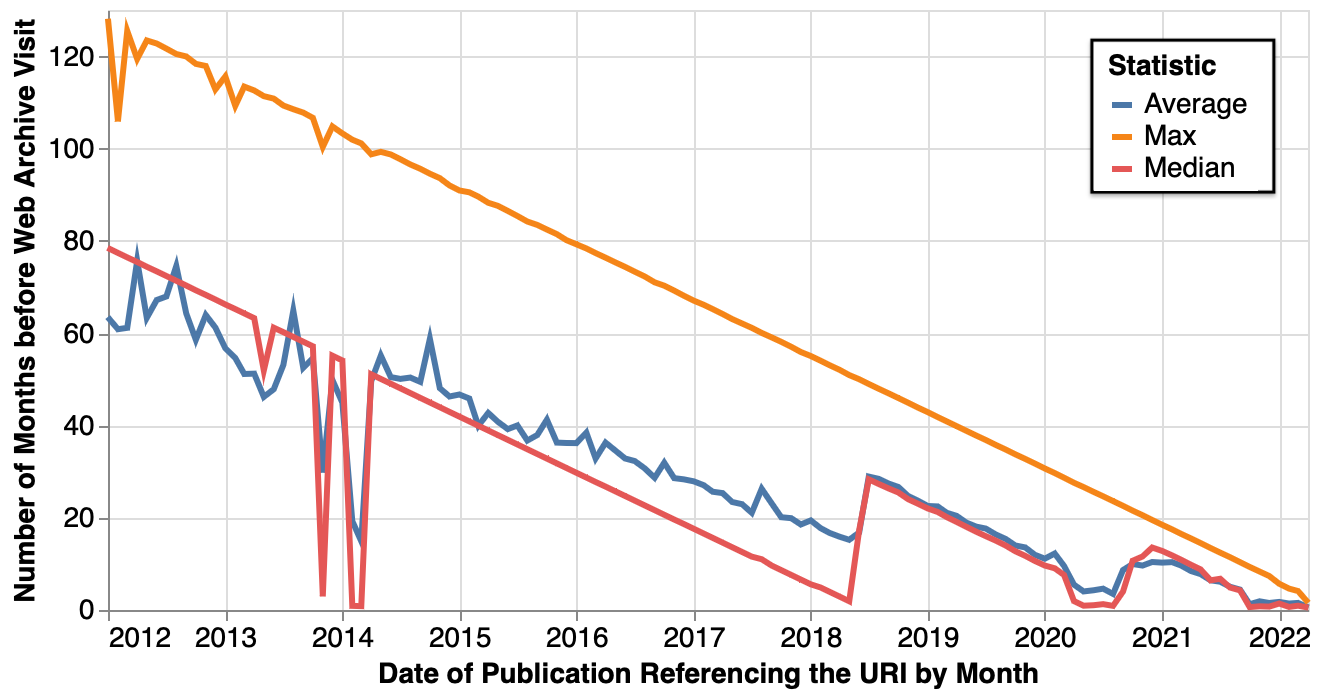
\includegraphics[width=0.85\linewidth]{archives_delta_over_time.png}
    \caption{Number of months between a publication referencing a URI and the URI being captured by the Web archives over time. Only includes URIs not captured by the Web archives before the publication date of the referencing article.}
    \label{fig:timemap_delta}
\end{figure}